En el dieño de convertidores \textit{buck} es necesario añadir una etapa intermedia entre la señal PWM y los \textit{gates} de los transistores MOSFET por varias razones. La primera de ellas es que la salida de dicha etapa no es capaz de alcanzar los niveles de tensión necesarios para poner a los transistores en modo saturación. Además, es necesario cargar y descargar los capaciotres de los MOSFET para que estos puedan abrirse o cerrarse, por lo que se requien picos de corriente para alimentarlos. Por último, es necesario asegurar que ambos MOSFET nunca estén abiertos a la vez, por lo que se necesita implementar un tiempo muerto entre la conmutación de ambas llaves. Estas tres funciones serán cumplidas por la etapa del \textit{gate driver}, la cual se implementa con el circuito integrado IR2104.

\begin{figure}[H]
    \centering
    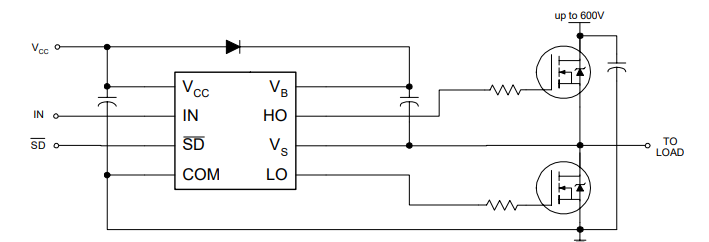
\includegraphics[width=0.8\textwidth]{img/gate driver/circuito GD.png}
    \caption{Circuito del \textit{gate driver}.}
    \label{fig:circuito GD}
\end{figure}

La \autoref{fig:circuito GD} fue extraída de la hoja de datos del integrado y muestra el circuito a implementar. El capacitor entre las entradas $V_B$ y $V_S$ es el capacitor de \textit{bootstrap}, el cual almacena la carga con la que se alimentará a los capacitores del MOSFET superior para que empiece a conducir. El diodo de \textit{bootstrap} permite que el capacitor se cargue a través de $V_{CC}$ en un semiciclo y fuerza a que su carga vaya al \textit{gate} en el otro. Por lo tanto, dicho diodo debe ser capaz de operar correctamente a la frecuencia de conmutación del circuito, por lo que se decidió utilizar los diodos Schottky antes mencionados (1N5822). 

El capacitor de \textit{bootstrap} no puede tener un valor arbitrario, debe tener un mínimo valor suficiente para cargar la compurta del transistor superior. Se impone entonces la siguiente restriccióna su capacidad:
\begin{equation*}
    C_{boot} > 10 \cdot \frac{Q}{V_{CC} - V_d} \,,
\end{equation*}
donde $Q$ es la carga de la compuerta del transistor y $V_d$ es la tensión de caída del diodo. Esta restricción asegura que el capacitor nunca se descargue completamente. De la hoja de datos del transistor se obtiene $Q = \SI{62}{\nano \coulomb}$, y con $V_{CC} = \SI{10}{\volt}$ y $V_d = \SI{0,2}{\volt}$ se tiene que $C_{boot} > \SI{63.2}{\nano \farad}$. De esta forma, se eligió $C_{boot} = \SI{100}{\nano \farad}$ para tener ciero margen.

A la hora de añadir el \textit{gate driver} a la placa fue necesario hacer modificaciones a la misma. Tanto el generador de  PWM como la etapa de compensación son alimentados por un regulador LM7809, el cual entrega $\SI{9}{\volt}$. Sin embargo, la hoja de datos del IR2104 informa que el mismo debe ser alimentado con $\SI{10}{\volt}$ o más, lo que fue comprobado experimentalmente.

\begin{minipage}{0.45\textwidth}
    \begin{figure}[H]
        \centering
        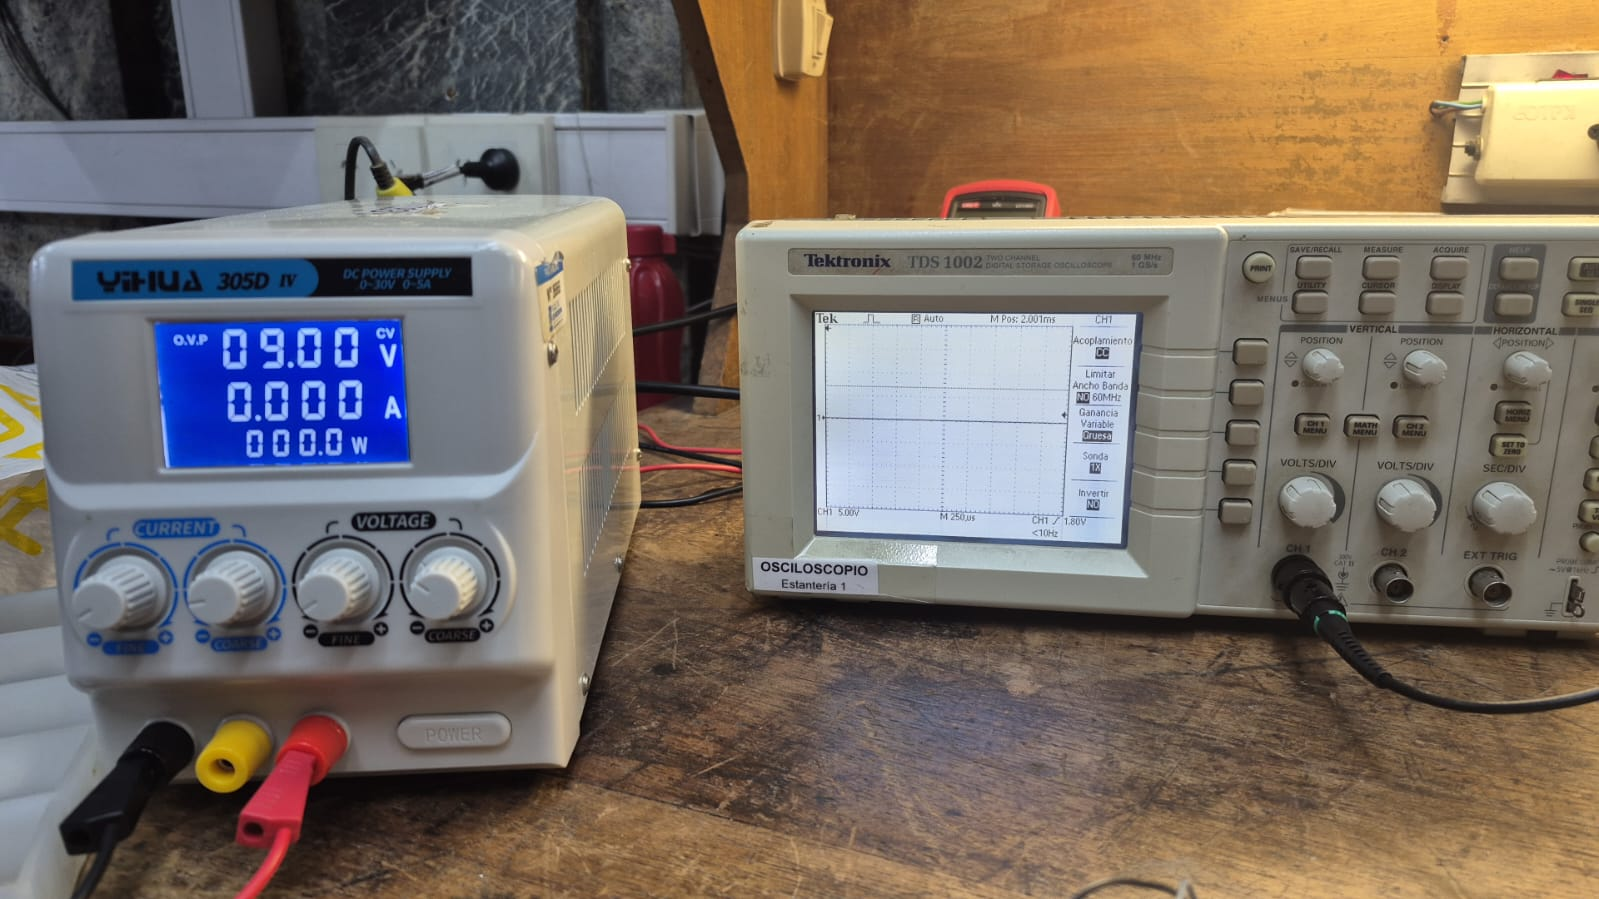
\includegraphics[width=0.9\textwidth]{img/gate driver/GD_9V.png}
        \caption{\textit{Gate driver} alimentado con $9\,$V.}
        \label{fig:GD 9V}
    \end{figure}
\end{minipage}
\begin{minipage}{0.45\textwidth}
    \begin{figure}[H]
        \centering
        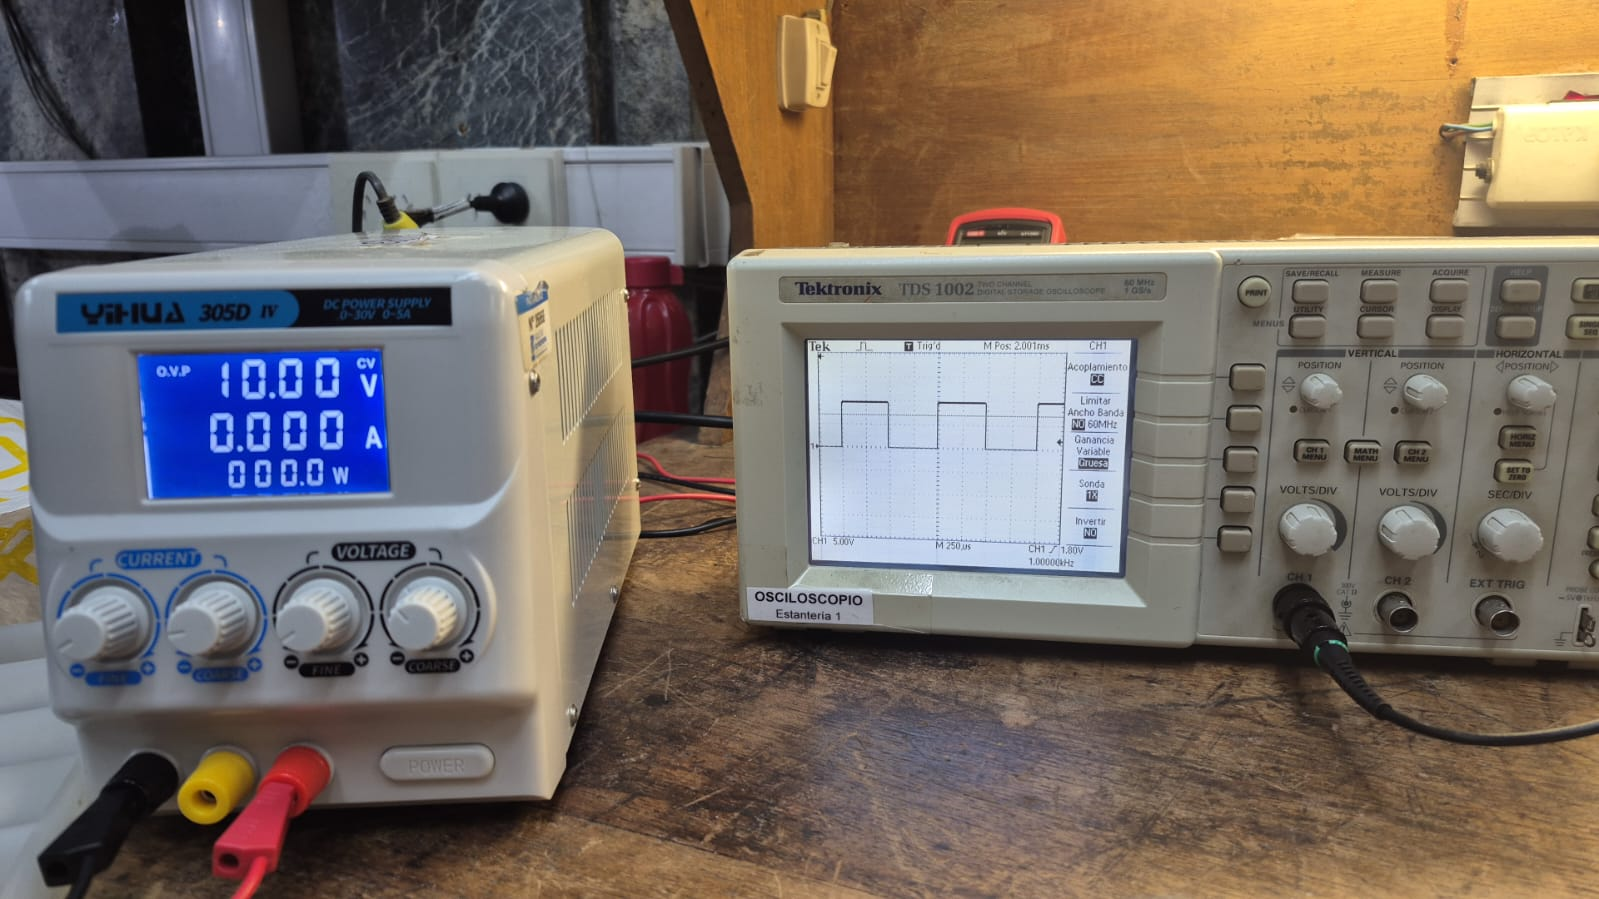
\includegraphics[width=0.9\textwidth]{img/gate driver/GD_10V.png}
        \caption{\textit{Gate driver} alimentado con $10\,$V.}
        \label{fig:GD 10V}
    \end{figure}
\end{minipage}

Se alimentó el \textit{gate driver} con $\SI{9}{\volt}$ y $\SI{10}{\volt}$ y se midió una de sus salidas con un osciloscopio. En las Figuras \ref{fig:GD 9V} y \ref{fig:GD 10V} se ecuentra el resultado del experimento, y puede comprobarse que en la pantalla del osciloscopio se obtiene una señal cuadrada a la salida solo si se alimenta al integrado con $\SI{10}{\volt}$ o más.
